\section{Loggable Class Reference}
\label{classLoggable}\index{Loggable@{Loggable}}
{\tt \#include $<$Loggable.hpp$>$}

Inheritance diagram for Loggable::\begin{figure}[H]
\begin{center}
\leavevmode
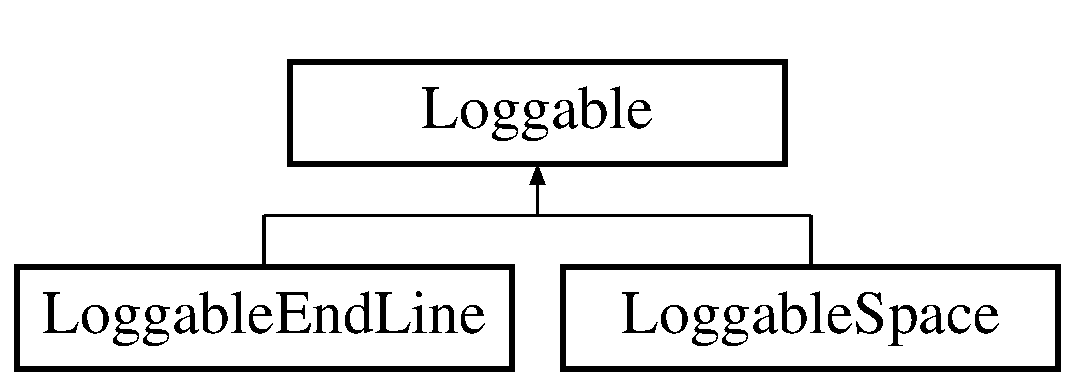
\includegraphics[height=2cm]{classLoggable}
\end{center}
\end{figure}
\subsection*{Public Member Functions}
\begin{CompactItemize}
\item 
virtual std::string {\bf to\-String} () const =0
\end{CompactItemize}


\subsection{Detailed Description}
Description: Loggable specifies an interface classes may inherit to more easily integrate with the {\bf Log\-Manager}{\rm (p.\,\pageref{classLogManager})}.



\subsection{Member Function Documentation}
\index{Loggable@{Loggable}!toString@{toString}}
\index{toString@{toString}!Loggable@{Loggable}}
\subsubsection{\setlength{\rightskip}{0pt plus 5cm}virtual std::string Loggable::to\-String () const\hspace{0.3cm}{\tt  [pure virtual]}}\label{classLoggable_a0}


Clients should use this interface memeber to provide the logger with a formatted message.

Implemented in {\bf Loggable\-End\-Line} {\rm (p.\,\pageref{classLoggableEndLine_a0})}, and {\bf Loggable\-Space} {\rm (p.\,\pageref{classLoggableSpace_a0})}.

The documentation for this class was generated from the following file:\begin{CompactItemize}
\item 
Loggable.hpp\end{CompactItemize}
